\chapter{Methodologies}

\label{chapter:methodologies}

In this chapter, we describe the methodologies used in this thesis.
Comprehensive source code reflecting these methodologies can be found in our
public GitHub
repository\footnote{https://github.com/atreyasha/spp-explainability}.

\section{Facebook Multilingual Task Oriented Dialog}

\citet{schuster-etal-2019-cross-lingual} originally released the Facebook
Multilingual Task Oriented Dialog (FMTOD) data set to encourage research in
cross-lingual transfer learning for Natural Language Understanding (NLU) tasks;
specifically from from high-resource to low-resource languages. The authors
released the FMTOD data set with English as the high-resource language providing
$\sim$43k annotated utterances, and Spanish and Thai as low-resource languages
providing a total of $\sim$14k utterances. Furthermore, they streamlined the
data set on two key tasks; namely intent detection and textual slot filling. In
this thesis, we focus solely on the English language intent detection task in
the FMTOD data set. This intent detection task entails a multi-label sequence
classification task with a total of 12 classes from alarm, reminder and
weather-related domains.

\subsection{Motivation}

We chose to work with the FMTOD data set since it is both a recently released
and well-studied data set
\citep{schuster-etal-2019-cross-lingual,zhang2019joint,zhang-etal-2020-intent}.
We focus on the English language intent classification task since it is a
relatively straightforward task which allows us to place a greater focus on
performance and explainability. Furthermore, the English language subset entails
the highest resources in the FMTOD data set. Finally, we find the FMTOD data
set's intent detection classification especially attractive because it allows us
to test the SoPa++ model on a multi-class NLU problem; which is significantly
different from the focus on binary classification sentiment detection tasks in
SoPa \citep{schwartz2018sopa}.

\subsection{Preprocessing}

We enumerate our preprocessing steps below:

\begin{enumerate}{}
  \item Similar to \citet{schwartz2018sopa}, we convert all FMTOD text samples
  to a lowercased format. This assists in simplifying the data set further.
  \item Next, we search through the pre-provided training, validation and test
  data partitions to remove duplicates within each partition.
  \item Finally, we remove data duplicates which overlap between partitions.
  During this step, we do not remove any cross-partition duplicates from the
  test partition in order to keep it as similar as possible to the original test
  partition. This comes into importance later when we compare performance
  evaluations on the test set with other studies.
\end{enumerate}

\begin{figure}[t]
  \centering
  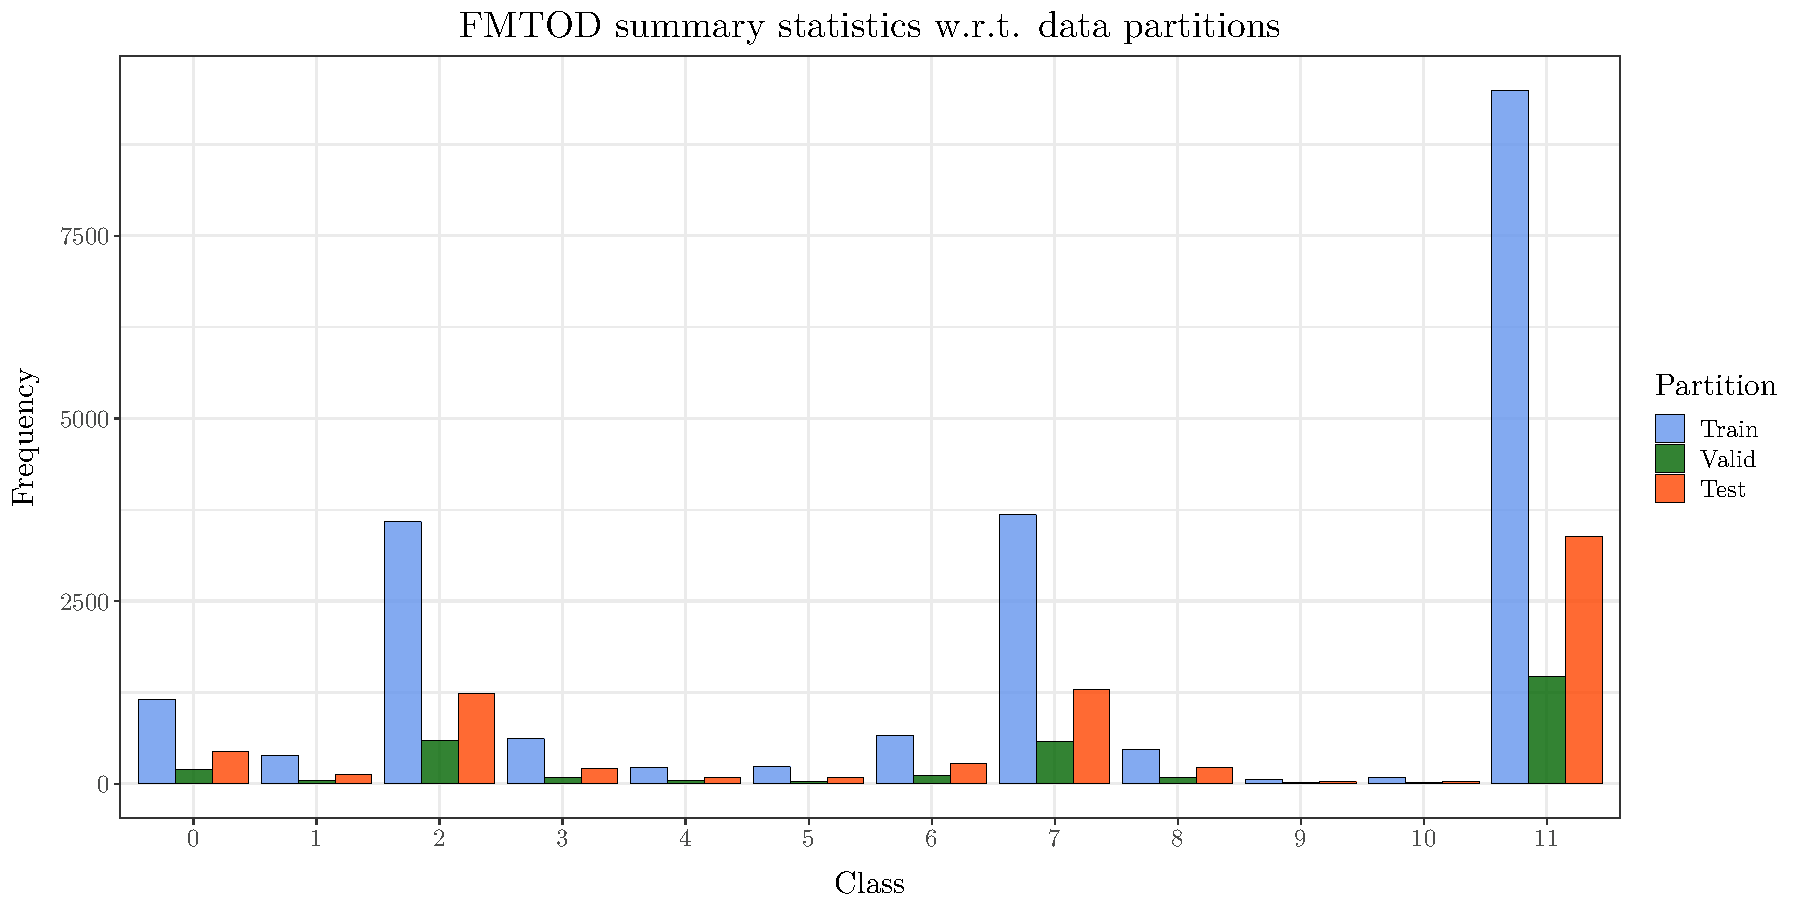
\includegraphics[width=14cm]{pdfs/generated/fmtod_summary_statistics.pdf}
  \caption{Data distribution of the preprocessed FMTOD data set grouped by
    classes and partitions}
  \label{fig:fmtod}
\end{figure}

\begin{table}[t!]
  \centering
  \begin{tabular}{lllll}
    \toprule
    Class and description & Train & Validation & Test & $\Sigma$ \\
    \midrule
    0: \texttt{alarm/cancel\_alarm} & 1157 & 190 & 444 & 1791 \\
    1: \texttt{alarm/modify\_alarm} & 393 & 51 & 122 & 566 \\
    2: \texttt{alarm/set\_alarm} & 3584 & 596 & 1236 & 5416 \\
    3: \texttt{alarm/show\_alarms} & 619 & 83 & 212 & 914 \\
    4: \texttt{alarm/snooze\_alarm} & 228 & 49 & 89 & 366 \\
    5: \texttt{alarm/time\_left\_on\_alarm} & 233 & 30 & 81 & 344 \\
    6: \texttt{reminder/cancel\_reminder} & 662 & 114 & 284 & 1060 \\
    7: \texttt{reminder/set\_reminder} & 3681 & 581 & 1287 & 5549 \\
    8: \texttt{reminder/show\_reminders} & 474 & 82 & 217 & 773 \\
    9: \texttt{weather/check\_sunrise} & 63 & 13 & 25 & 101 \\
    10: \texttt{weather/check\_sunset} & 88 & 11 & 37 & 136 \\
    11: \texttt{weather/find} & 9490 & 1462 & 3386 & 14338 \\[5pt]
    \hline \hline \\[-10pt]
    $\Sigma$ & 20672 & 3262 & 7420 & 31354 \\
    \bottomrule
  \end{tabular}
  \caption{Frequency of the preprocessed FMTOD data set classes grouped by
    partitions; $\Sigma$ signifies the cumulative frequency statistic}
  \label{tab:fmtod}
\end{table}

Many of the duplicates observed were already present in the original FMTOD data
set, with additional duplicates being created from the initial lowercasing step.
After preprocessing, we obtain a lowercased variant of the FMTOD data set with
strictly unique data partitions. In the next section, we describe the summary
statistics of the preprocessed FMTOD data set.

\begin{table}[t!]
  \centering
  \begin{threeparttable}
    \begin{tabular}{lll}
      \toprule
      Class and description & Utterance length$^{\dagger}$ & Example$^{\ddagger}$ \\
      \midrule
      0: \texttt{alarm/cancel\_alarm} & 5.6 $\pm$ 1.9 & cancel weekly alarm \\
      1: \texttt{alarm/modify\_alarm} & 7.1 $\pm$ 2.5 & change alarm time \\
      2: \texttt{alarm/set\_alarm} & 7.5 $\pm$ 2.5 & please set the new alarm \\
      3: \texttt{alarm/show\_alarms} & 6.9 $\pm$ 2.2 & check my alarms. \\
      4: \texttt{alarm/snooze\_alarm} & 6.1 $\pm$ 2.1 & pause alarm please \\
      5: \texttt{alarm/time\_left\_on\_alarm} & 8.6 $\pm$ 2.1  & minutes left on my alarm \\
      6: \texttt{reminder/cancel\_reminder} & 6.6 $\pm$ 2.2 & clear all reminders. \\
      7: \texttt{reminder/set\_reminder} & 8.9 $\pm$ 2.5 & birthday reminders \\
      8: \texttt{reminder/show\_reminders} & 6.8 $\pm$ 2.2 & list all reminders \\
      9: \texttt{weather/check\_sunrise} & 6.7 $\pm$ 1.7 & when is sunrise \\
      10: \texttt{weather/check\_sunset} & 6.7 $\pm$ 1.7 & when is dusk \\
      11: \texttt{weather/find} & 7.8 $\pm$ 2.3 & jacket needed? \\[5pt]
      \hline \hline \\[-10pt]
      $\mu$ & 7.7 $\pm$ 2.5 & \textemdash \\
      \bottomrule
    \end{tabular}
    \begin{tablenotes}[flushleft]
      \footnotesize
      \item $^{\dagger}$Summary statistics follow the mean $\pm$
      standard-deviation format
      \item $^{\ddagger}$Short and simple examples were chosen for brevity and
      formatting purposes
    \end{tablenotes}
  \end{threeparttable}
  \caption{Tabular summary of utterance length statistics and examples for FMTOD
    data classes; $\mu$ signifies the cumulative summary statistics}
  \label{tab:fmtod_examples}
\end{table}

\begin{table}[t!]
  \centering \def\arraystretch{1.3}
  \begin{tabular}{L{0.27\linewidth} L{0.45\linewidth} l}
    \toprule
    Study & Summary & Accuracy \\
    \midrule
    \citet{schuster-etal-2019-cross-lingual} & BiLSTM jointly trained on both the slot filling and intent detection English language tasks & 99.1$\%$ \\
    \citet{zhang2019joint} & BERT along with various decoders jointly fine-tuned on both the slot filling and intent detection English language tasks & 96.6--98.9$\%$ \\
    \citet{zhang-etal-2020-intent} & RoBERTa and XLM-RoBERTa fine-tuned on the English language and multilingual intent detection tasks respectively along with WikiHow pre-training & 99.3--99.5$\%$ \\
    \bottomrule
  \end{tabular}
  \caption{Tabular summary of studies that addressed the FMTOD intent detection
    English language task, along with their relevant summaries and accuracy
    range(s)}
  \label{tab:fmtod_results}
\end{table}

\subsection{Summary statistics}

Figure \ref{fig:fmtod} shows the summary statistics of the preprocessed FMTOD
data set grouped by classes and data set partitions. Similarly, Table
\ref{tab:fmtod} shows the same summary statistics in a tabular form with
explicit frequencies. Based on the summary statistics, we can observe that the
preprocessed FMTOD data set is significantly imbalanced with $\sim$45$\%$ of
samples falling into Class 11 alone. We take this observation into consideration
in later sections and apply fixes to mitigate this data imbalance. In addition,
we observe from Table \ref{tab:fmtod_examples} that input utterances in the
preprocessed FMTOD data set are generally short; with a mean input utterance
length of 7.7 and a standard deviation of 2.5 tokens. Utterance length summary
statistics were computed with the assistance of NLTK's default \texttt{Treebank}
word tokenizer \citep{bird-loper-2004-nltk}.

\subsection{Performance range}

Several studies have optimized deep learning models on the FMTOD English
language intent classification task using a variety of models from BiLSTMs to
XLM-RoBERTa
\citep{schuster-etal-2019-cross-lingual,zhang2019joint,zhang-etal-2020-intent}.
Table \ref{tab:fmtod_results} summarizes these studies along with their reported
accuracy scores on the FMTOD English language intent classification task. Based
on the presented results from these recent studies, we can infer that the
general competitive accuracy range for the FMTOD English language intent
classification task is from 96.6$\%$ to 99.5$\%$.

\section{SoPa++}

In this section we describe our SoPa++ model's architecture and present both
similarities and differences compared to the SoPa model in
\citet{schwartz2018sopa}.

\subsection{Strict linear-chain WFA-$\omega$}

As mentioned in Section \ref{section:sopa}, \citet{schwartz2018sopa}
constructed the SoPa model with an ensemble of linear-chain WFAs which permitted
both $\epsilon$ and self-loop transitions. As noted in Section
\ref{section:sopa_cg}, $\epsilon$ and self-loop transitions are useful
constructs in abstracting WFAs and allowing them to consume or match variable length
strings. However based on our experimentation during our development phase, we
observed a key concern that the highest scoring paths in the WFAs in SoPa tended
to have a large variation of string lengths due to the effect of both
$\epsilon$-transitions and self-loops. We believe that this reduced the impact of
SoPa's explainability methods and as a result, the first change we decided for
was to remove both $\epsilon$ and self-loop transitions. With this change, we could
at least ensure that each WFA would always consume strings of fixed lengths.

However, consuming strings of fixed lengths could also be seen as a form of
overfitting in the model; since a model could simply memorize short strings or
phrases and would not necessarily "learn" to generalize. To address this
concern, we include a wildcard transition which we define here as a
$\omega$-transition. Allowing for such a transition was only natural since
wildcards are already crucial parts of regular expressions; which as we
mentioned are equivalent to FAs. To support this, we provide the following
definition for a modified WFA-$\omega$:

\begin{definition}[Weighted finite-state automaton-$\omega$]
  \label{def:wfa_w}
  A weighted finite-state automaton-$\omega$ over a semiring $\mathbb{K}$ is a
  5-tuple $\mathcal{A} = \langle \Sigma, \mathcal{Q}, \bm{\Gamma}, \bm{\lambda}, \bm{\rho}
  \rangle$, with:

  \begin{itemize}
  \itemsep0em
    \item[--] a finite input alphabet $\Sigma$;
    \item[--] a finite state set $\mathcal{Q}$;
    \item[--] transition matrix $\bm{\Gamma}: \mathcal{Q} \times \mathcal{Q} \times (\Sigma \cup \{\omega\}) \rightarrow \mathbb{K}$;
    \item[--] initial vector $\bm{\lambda}: \mathcal{Q} \rightarrow \mathbb{K}$;
    \item[--] and final vector $\bm{\rho}: \mathcal{Q} \rightarrow \mathbb{K}$.
  \end{itemize}

  \begin{remark}
    An $\omega$ transition is equivalent to a wildcard transition, which
    consumes an arbitrary token input and moves to the next state
  \end{remark}

  \begin{remark}
    Besides the inclusion of the $\omega$-transition and removal of the
    $\epsilon$-transition, an WFA-$\omega$ has all of the same characteristics
    as the WFA defined in Definition \ref{def:wfa}.
  \end{remark}
\end{definition}

Comparing with the linear-chain WFAs used in \citet{schwartz2018sopa} as
mentioned in Section \ref{section:sopa_lc_wfa}, our linear-chain WFA-$\omega$ is
similarly alloted a sequence of $|\mathcal{Q}|$ states. However, each state $i$
in the linear-chain WFA-$\omega$ has only two possible outgoing transitions;
namely a \textbf{$\omega$-transition} which consumes an arbitrary input token
and transitions to state $i+1$ and a \textbf{main-path transition} which
consumes a specific token and transitions to state $i+1$. Similar to
\citet{schwartz2018sopa}, we utilize only the max-sum and max-product semirings
in our linear-chain WFA-$\omega$'s. Because of the elimination of self-loop
transitions, we refer to our linear-chain WFA-$\omega$ as \textit{strict}
linear-chain WFA-$\omega$ as per Definition \ref{def:lfa}. 

\begin{figure}[t!]
  \centering
  \includegraphics[width=14cm]{pdfs/generated/w_nfa_linear_chain/main.pdf}
  \caption{Schematic visualizing a strict linear-chain NFA with
    $\omega$ (blue) and main-path (black) transitions}
  \label{fig:omega_fa}
\end{figure}

Next, we provide a mathematical formulation of the modified transition matrix
$\bm{\Gamma}$ in our linear-chain WFA-$\omega$. Here, $\bm{\Gamma}(x)$ represents a
$|Q|\times|Q|$ matrix containing transition scores when consuming an input token
$x$. $[\bm{\Gamma}(x)]_{i,j}$ corresponds to the cell value in $\bm{\Gamma}(x)$ for row
$i$ and column $j$ and represents the transition score when consuming token $x$
and transitioning from state $i$ to $j$.

\begin{equation}
  \label{eq:spp_transition_matrix_main}
  [\bm{\Gamma}(x)]_{i,j} =
  \begin{cases}
    \bm{w}_i \cdot \bm{v}_x + b_i  & \text{if } j = i + 1 \text{ (main-path transition),} \\
    \bar{0} & \text{otherwise.}
  \end{cases}
\end{equation}

Here, $\bm{w}_i$ and $b_i$ are learnable vector and scalar parameters
parameterizing transitions out of state $i$ to state $i+1$. $\bm{v}_x$
represents the word embedding for token $x$ and $\bar{0}$ represents the zero
value in the semiring used (Definition \ref{def:semiring}). Similarly,
$\omega$-transitions are parameterized with the following representation in
$\bm{\Gamma}$:

\begin{equation}
  \label{eq:spp_transition_matrix_omega}
  [\bm{\Gamma}(\omega)]_{i,j} =
  \begin{cases}
    c_i  & \text{if } j = i + 1 \text{ ($\omega$-transition)} \\
    \bar{0} & \text{otherwise.}
  \end{cases}
\end{equation}

Here, $c_i$ represents a learnable scalar bias for $\omega$-transitions out of
state $i$ to state $i+1$. Finally as per \citet{schwartz2018sopa}, we fix the
initial vector $\bm{\lambda} = [\bar{1}, \bar{0}, \ldots, \bar{0}]$ and the final
vector $\bm{\rho} = [\bar{0}, \bar{0}, \ldots, \bar{1}]$, where $\bar{1}$ and
$\bar{0}$ represent the one and zero values specified in the semiring
(Definition \ref{def:semiring}). The time-complexity of the Viterbi algorithm to
compute the string score for our linear-chain WFA-$\omega$'s is
$O(|Q||\bm{x}|)$, where $|\mathcal{Q}|$ refers to the number of states and
$|\bm{x}|$ refers to the length of the input string.

Ultimately, the introduction of a strict linear-chain WFA-$\omega$ allows us to
attain fixed string length consumption with an added layer of generalization
because of the introduction of wildcards. An example of a strict linear-chain
NFA extracted from a strict linear-chain WFA-$\omega$ is shown in Figure
\ref{fig:omega_fa}. Interestingly, we can observe that this FA corresponds to
the Perl-compatible regular expression \texttt{``what a (great|entertaining)
  [\^{}\textbackslash\textbackslash s]+ !''}, where
\texttt{[\^{}\textbackslash\textbackslash s]+} refers to any set of consecutive
characters which are not separated by a space character.

\begin{algorithm}[t!]
  \small
  \caption{Strict linear-chain WFA-$\omega$ document score$^*$}
  \label{algo:lc_wfa_w_document_score}
  \begin{algorithmic}[1]
    \Require{Strict linear-chain WFA-$\omega$ and document $\bm{y}$}
    \Ensure{Document score $s_{\text{doc}}(\bm{y})$}
    \Statex
    \Begin
    \State $\bm{h}_0 \gets \big[\bar{1}, -\infty, \ldots, -\infty\big]$ \Comment{Create
      initial hidden state vector $\bm{h}_0: \mathcal{Q} \rightarrow \mathbb{K}$}
    \For{$i \gets 1,2,\ldots,\bm{|y|}$} \Comment{Sequentially iterate over each
      token $y_i$ in string $\bm{y}$}
    \State $\bm{m} \gets \big[[\bm{\Gamma}(y_i)]_{1,2}, [\bm{\Gamma}(y_i)]_{2,3}, \ldots,
    [\bm{\Gamma}(y_i)]_{|\mathcal{Q}|-1,|\mathcal{Q}|}\big]$ \Comment{Main-path scores for token $y_i$}
    \State $\bm{\omega} \gets \big[[\bm{\Gamma}(\omega)]_{1,2}, [\bm{\Gamma}(\omega)]_{2,3}, \ldots,
    [\bm{\Gamma}(\omega)]_{|\mathcal{Q}|-1,|\mathcal{Q}|}\big]$
    \Comment{State-wise wildcard scores}
    \State $\bm{m'} \gets \bm{m} \otimes \bm{h}_{i-1}[:-1]$ \Comment{Path
      score with main-path transitions$^{\dagger}$}
    \State $\bm{\omega'} \gets \bm{\omega} \otimes \bm{h}_{i-1}[:-1]$ \Comment{Path
    score with $\omega$ transitions$^{\dagger}$}
    \State $\bm{h}_{i} \gets [\bar{1}] \mathbin\Vert \max(\bm{m'}, \bm{w'})$
    \Comment{Concatenate $\bar{1}$ to maximum of $\bm{m}$ and $\bm{\omega}$}
    \EndFor
    \State $s_{\text{doc}}(\bm{y}) \gets  \max_{i \in 1,2,...,|\bm{y}|}
    \bm{h}_{i}[-1]$
    \Comment{Get maximum of hidden vector final states$^{\ddagger}$}
    \State \Return $s_{\text{doc}}(\bm{y})$
    \End
  \end{algorithmic}
  \algcomment{
    $^*$$\otimes$ and $\bar{1}$ are
    derived from max-based semirings where all semiring operations are element-wise \\
    $^{\dagger}\bm{h}_{i}[:-1]$ follows the Python indexing syntax
    and implies keeping all elements of $\bm{h}_{i}$ except the last \\
    $^{\ddagger}\bm{h}_{i}[-1]$ follows the Python indexing syntax and implies
    retrieving the last element of the vector $\bm{h}_{i}$
  }
\end{algorithm}

\subsection{Document score}

Similar to \citet{schwartz2018sopa}, SoPa++ was intended to compute scores for
entire documents and not just fixed-length strings using the strict linear-chain
WFA-$\omega$. To achieve this, we propose Algorithm
\ref{algo:lc_wfa_w_document_score} to compute the document score
$s_{\text{doc}}(\bm{y})$ for an arbitrary document $\bm{y}$. Here, we score all
consecutive substrings in a document $\bm{y}$ using either the max-sum or
max-product semirings assisted with the Viterbi algorithm. Following from this,
the document score $s_{\text{doc}}(\bm{y})$ for an arbitrary document $\bm{y}$
would reflect the highest scoring path which corresponds to the a substring in
document $\bm{y}$.

\subsection{TauSTE}

In Section \ref{section:ste} we described the concept of a STE in activation
quantized neural networks and explained how STEs function in both their forward
and backward passes. Furthermore, we provided a motivation as to why STEs and
other quantized activation functions are of interest; for example in relation to
computational savings linked to low-precision computing. In our implementation
of the SoPa++ model, we make use of a variant of the STE activation function;
which we define here as the Tau straight-through estimator (TauSTE).

\begin{equation}
  \label{eq:tau_ste_forward}
  \text{TauSTE}(x)=
  \begin{cases}
    1 & x \in (\tau, +\infty) \\
    0 & x \in (-\infty, \tau]
  \end{cases}
\end{equation}

\begin{equation}
  \label{eq:tau_ste_backward}
  \text{TauSTE}'(x)=
  \begin{cases}
    1 & x \in  (1, +\infty) \\
    x & x \in [-1, 1] \\
    -1 & x \in (-\infty, -1) \\
  \end{cases}
\end{equation}

\begin{figure}[t!]
  \centering
  \includegraphics[width=14cm]{pdfs/generated/tau_ste_applied/main.pdf}
  \caption{Schematic visualizing the TauSTE's forward and backward passes}
  \label{fig:tau_ste}
\end{figure}

Figure \ref{fig:tau_ste} shows a schematic of the TauSTE's forward and backward
passes. As we can see, there are two key changes from the vanilla STE to the
TauSTE. Firstly, the threshold for activation in the forward function is now
governed by some variable $\tau \in \mathbb{R}$. This was done to allow for some
degree of freedom in deciding the activation threshold. Secondly, the backward
pass returns the identity function on a limited range on inputs; specifically on
$x \in [-1,1]$. This restriction on the backward pass was placed to ensure that
gradients do not blow up in size.

As we describe in detail in the next sections, we chose to use this special
variant of the STE because we believe that the TauSTE could prove to be useful
for the explainability purposes of our SoPa++ model. This is mainly because the
TauSTE (or even the STE) activation function simplifies continuous inputs into
discrete outputs; thereby reducing the information content of the signal it
receives as inputs. In later sections, we show how we utilize and capitalize
this reduction in signal information in our SoPa++ model.

\subsection{Tokenization and embeddings}

Similar to \citet{schwartz2018sopa}, we utilize NLTK's default \texttt{Treebank}
word tokenizer \citep{bird-loper-2004-nltk} to conduct tokenization of input
utterances into word-level tokens. Next, we pad input utterances with special
\texttt{[START]} and \texttt{[END]} tokens at the start and end indices of the
utterances to signify the location where the utterance begins and ends. Finally,
while \citet{schwartz2018sopa} utilize GloVe 840B 300-dimensional true-cased
embeddings, we utilize GloVe 6B 300-dimensional uncased word-level embeddings
\citep{pennington2014glove} to project the input tokens in utterances to
continuous numerical spaces. We utilized this smaller subset of word-level
embeddings since it allowed us to work with lower-cased words, as well as
experiment with a variety of embedding dimensions during our development phase.

\begin{figure}[t!]
  \centering
  \includegraphics[width=15cm]{pdfs/generated/spp_computational_graph/main.pdf}
  \caption{Schematic visualizing the computational graph of the SoPa++ model}
  \label{fig:spp_cg}
\end{figure}

\subsection{Computational graph}

In this subsection, we describe the computational graph of the SoPa++ model by
specifically referring to its several neural components. This description is
linked to the visualization of the computational graph of SoPa++ in Figure
\ref{fig:spp_cg}. Firstly as described in the previous section, we tokenize the
input utterance, pad it with special tokens and project input tokens to
numerical spaces using the aforementioned GloVe word embeddings. Following this,
we use our ensemble of $m \in \mathbb{N}$ strict linear-chain WFA-$\omega$'s to
traverse the input utterance and provide an ultimate document score for this
utterance; as prescribed by Algorithm \ref{algo:lc_wfa_w_document_score}. When
processing each input token, we monitor the end states of each of the $m \in
\mathbb{N}$ WFA-$\omega$ and max-pool the score present in this state. In the
edge case that an input string was too short for the end state of WFA-$\omega$
to register a non-$\bar{0}$ score, we simply discard this score in further
analysis. This description so far corresponds to the lower half of Figure
\ref{fig:spp_cg}.

After max-pooling scores from all the $m \in \mathbb{N}$ WFA-$\omega$'s, we
then pass this collection of pattern scores for further processing using SoPa++'s other
neural components. This can be seen in the upper portion of Figure
\ref{fig:spp_cg}. Firstly, we apply layer normalization \citep{ba2016layer} to
all pattern scores without applying any additional affine
transformations. We omit the affine transformation to not alter any of the
pattern score information content and use layer normalization as an expedient
means of projecting the values of pattern scores to a standard normal
distribution. This furthermore guarantees that pattern scores would be
smaller in size and would have a roughly even distribution of small positive and
negative values around 0.

This projection to a standard normal distribution becomes very useful as we next
encounter the TauSTE layer. Here, this layer maps all inputs which are strictly
larger than the $\tau \in \mathbb{R}$ threshsold to 1 and all others inputs to
zero. The TauSTE layer naturally is only useful when it is able to discriminate
the inputs by mapping some of them to 1 and some to 0, instead of always mapping
all inputs to either 1 or 0. Without layer normalization, the TauSTE layer would
not be able to perform its function since pattern scores tend to be mostly
positive with differing ranges. Layer normalization therefore helps to project
these variations of scores to a uniform range; which ultimately allows the
TauSTE layer to be useful.

A natural criticism of the TauSTE layer could be that it strongly limits the
flow of information in the SoPa++ model. While the binarization present in this
layer does indeed limit the rich flow of continuous numerical information, it is
still worth noting that this layer can preserve sufficient information given a
sufficiently large $m \in \mathbb{N}$ value and therefore number of WFA-$\omega$
and TauSTE neurons. For example, if we allow for $m=40$ and therefore provide 40
WFA-$\omega$ and TauSTE neurons, we can have a total of
2$^{40}\approx1.1\times10^{12}$ binary state possibilities; which is slightly
greater than one trillion state possibilities. To provide some context to this
order of magnitude, the aforementioned number of possibilities is roughly equal
to estimated number of stars present in the Andromeda Galaxy
\citep{10.1093/mnras/stu879}. This would imply that despite the reduction in
information content on the TauSTE layer, there are still sufficient mappable
states available to learn various representations relevant to output classes.

After binarizing the input values in the TauSTE layer, we apply a simple linear
or affine transformation to the inputs to modify their dimensionality from $m
\in \mathbb{N}$ to $n \in \mathbb{N}$, where the $n$ represents the number of
output classes. We specifically chose a linear regression layer over a MLP
because linear regressors are known to be transparent models
\citep{arrieta2020explainable} and this is a feature which ultimately assists us
in the explainability portion of the SoPa++ model, which we describe in greater
detail in the next sections.

Finally, after applying the linear transformation; we apply a softmax function
over the linear outputs to project them to probabalistic spaces and then extract
the highest scoring index to represent the predicted class. In the case of
Figure \ref{fig:spp_cg}, the output class for the input pre-processed sentence
\texttt{``[START] 10 day weather forecast [END]''} is the \texttt{weather/find} label
which corresponds to class 11.

\subsection{Transparency}

Similar to the SoPa model as mentioned in Section
\ref{section:sopa_transparency}, SoPa++ is also a hybrid model consisting of
RNN, CNN and weighted finite-state neural components. Following the standards of
transparency recommended by \citet{arrieta2020explainable}, we can conclude that
SoPa++ would correspondingly fall into the black-box ML model category. Because
of this classification, the SoPa++ model would require post-hoc explainability
methods in order to explain its inner mechanisms. In the next section, we
expound more on the explanations by simplification post-hoc explainability
method that can be used on the SoPa++ model.

\section{RE proxy}

In Section \ref{section:xai_techniques} we introduced three important post-hoc
explainability techniques; specifically local explanations, feature relevance
and explanations by simplification. In this section, we describe how we leverage
the latter explanations by simplifications technique with our SoPa++ model.
Specifically, we show how we can use special features of the antecedent SoPa++
model to effectively simplify it into a Regular Expression (RE) proxy model.

\subsection{Document score with corresponding path}

\begin{algorithm}[t!]
  \small
  \caption{Strict linear-chain WFA-$\omega$ document score with corresponding path$^*$}
  \label{algo:lc_wfa_w_document_score_trace}
  \begin{algorithmic}[1]
    \Require{Strict linear-chain WFA-$\omega$ and document $\bm{y}$}
    \Ensure{Document score $s_{\text{doc}}(\bm{y})$ and its corresponding path $\pi_{\text{doc}}(\bm{y})$}
    \Statex
    \Begin
    \State $\bm{h}_0 \gets \big[\bar{1}, -\infty, \ldots, -\infty\big]$ \Comment{Create
      initial hidden state vector $\bm{h}_0: \mathcal{Q} \rightarrow \mathbb{K}$}
    \For{$i \gets 1,2,\ldots,\bm{|y|}$} \Comment{Sequentially iterate over each
      token $y_i$ in string $\bm{y}$}
    \State $\bm{m} \gets \big[[\bm{\Gamma}(y_i)]_{1,2}, [\bm{\Gamma}(y_i)]_{2,3}, \ldots,
    [\bm{\Gamma}(y_i)]_{|\mathcal{Q}|-1,|\mathcal{Q}|}\big]$ \Comment{Main-path scores for token $y_i$}
    \State $\bm{\omega} \gets \big[[\bm{\Gamma}(\omega)]_{1,2}, [\bm{\Gamma}(\omega)]_{2,3}, \ldots,
    [\bm{\Gamma}(\omega)]_{|\mathcal{Q}|-1,|\mathcal{Q}|}\big]$
    \Comment{State-wise wildcard scores}
    \State $\bm{m'} \gets \bm{m} \otimes \bm{h}_{i-1}[:-1]$ \Comment{Path
      score with main-path transitions$^{\dagger}$}
    \State $\bm{\omega'} \gets \bm{\omega} \otimes \bm{h}_{i-1}[:-1]$ \Comment{Path
    score with $\omega$ transitions$^{\dagger}$}
    \State $\bm{h}_{i} \gets [\bar{1}] \mathbin\Vert \max(\bm{m'}, \bm{w'})$
    \Comment{Concatenate $\bar{1}$ to maximum of $\bm{m}$ and $\bm{\omega}$}
    \State $\pi_i \gets \text{trace}(h_i[-1])$
    \Comment{Back-trace path $\pi_i$ corresponding to $h_i[-1]^{\ddagger}$}
    \EndFor
    \State $j \gets \argmax_{i \in 1,2,...,|\bm{y}|}
    \bm{h}_{i}[-1]$
    \Comment{Get index of hidden vector final states' maximum$^{\ddagger}$}
    \State $s_{\text{doc}}(\bm{y}) \gets \bm{h}_{j}[-1]$
    \Comment{Extract maximum hidden vector final state value$^{\ddagger}$}
    \State $\pi_{\text{doc}}(\bm{y}) \gets \pi_j$
    \Comment{Extract path corresponding to maximum value}
    \State \Return $\{s_{\text{doc}}(\bm{y}), \pi_{\text{doc}}(\bm{y})\}$
    \End
  \end{algorithmic}
  \algcomment{
    $^*$$\otimes$ and $\bar{1}$ are
    derived from max-based semirings where all semiring operations are element-wise \\
    $^{\dagger}\bm{h}_{i}[:-1]$ follows the Python indexing syntax
    and implies keeping all elements of $\bm{h}_{i}$ except the last \\
    $^{\ddagger}\bm{h}_{i}[-1]$ follows the Python indexing syntax and implies
    retrieving the last element of the vector $\bm{h}_{i}$
  }
\end{algorithm}

As described in Definition \ref{def:string_score}, the Viterbi algorithm returns
the highest path score which can naturally be attributed to a certain path or
set of transitions. In order to simplify the SoPa++ model into a RE proxy model,
we first need to modify our document scoring algorithm to not only return the
document score $s_{\text{doc}}(\bm{y})$ but also its corresponding path
$\pi_{\text{doc}}(\bm{y})$. This process is described in Algorithm
\ref{algo:lc_wfa_w_document_score_trace} where we trace the exact path of each
transition and return the exact path in addition to the highest path-score. This
algorithm ultimately allows us to extract the highest scoring path for each
strict linear-chain WFA-$\omega$ used in SoPa++ per input utterance. Similar to
Algorithm \ref{algo:lc_wfa_w_document_score}, this algorithm also has a
time-complexity of $O(|Q||\bm{x}|)$, where $|\mathcal{Q}|$ refers to the number
of states and $|\bm{x}|$ refers to the length of the input string. It is also
worth noting that the highest scoring path returned ultimately reflects a set of
transitions in the form of a strict linear-chain NFA; which can correspondingly
be transformed into a regular expression. Therefore, it can be inferred that
Algorithm \ref{algo:lc_wfa_w_document_score_trace} returns the best scoring
regular expression corresponding to a certain strict linear-chain WFA-$\omega$.

\subsection{Simplifying SoPa++ to RE proxy}

We now describe the simplification process from a neural SoPa++ model into a RE
proxy model. First, we assume that already have a fully trained SoPa++ model
given a certain task. We leave the details of training to the next sections.
With this trained SoPa++ model, we pass the model its training data again and
this time use Algorithm \ref{algo:lc_wfa_w_document_score_trace} to retrieve the
best scoring paths for each of the $m \in \mathbb{N}$ strict linear-chain
WFA-$\omega$'s in the SoPa++ model. This would imply that for each input
utterance in the training set, we collect the $m$ best path transitions for the
$m$ WFA-$\omega$'s, with each best path corresponding to a regular expression.
Naturally, not all best paths and regular expressions were important for the
classification decision of the antecedent SoPa++ model. Specifically, only the
regular expressions corresponding to activated TauSTE neurons were of importance
to the decision of the antecedent SoPa++ model; while all other regular
expressions were effectively discarded at the TauSTE layer.

This leads us to several interesting conclusions. Firstly, we observe here that
the TauSTE layer is not only useful for reducing information complexity; but
also for attributing causal links to the model's decision-making. This is shown
by the layer effectively reducing complexity and attributing the decision-making
process to certain regular expressions. Next, we can also observe an effect of
the $\tau \in \mathbb{R}$ threshold here. If the $\tau$-threshold is low, we
effectively allow more TauSTE neurons to be activated and therefore allow more
regular expressions from the strict linear-chain WFA-$\omega$ to affect the
SoPa++ model's final decision. Contrastingly, if the $\tau$-threshold is high;
we allow fewer TauSTE neurons to be activated and therefore allow fewer regular
expressions to be used for the final decision making process. Therefore, we can
infer that the TauSTE operates as a filtration layer which allows us to
construct causal links to simplify the SoPa++ model into a RE proxy model.

%%% Local Variables: 
%%% mode: latex
%%% TeX-master: "main"
%%% End: 